\documentclass[11pt,a4paper,fontset=fandol]{ctexart}

\usepackage[a4paper,margin=2.15cm]{geometry}
\usepackage{graphicx}
\usepackage{float}
\usepackage{booktabs}
\usepackage{longtable}
\usepackage{array}
\usepackage{xcolor}
\usepackage{hyperref}
\usepackage{tikz}
\usepackage{enumitem}
\usepackage{listings}
\usetikzlibrary{arrows.meta,positioning,shapes.geometric,calc}

\definecolor{blue}{HTML}{2563EB}
\definecolor{green}{HTML}{059669}
\definecolor{orange}{HTML}{D97706}
\definecolor{red}{HTML}{DC2626}
\definecolor{paper}{HTML}{F8FAFC}
\definecolor{line}{HTML}{CBD5E1}
\definecolor{softyellow}{HTML}{FEF3C7}
\definecolor{softgreen}{HTML}{DCFCE7}
\definecolor{softblue}{HTML}{DBEAFE}

\hypersetup{
  colorlinks=true,
  linkcolor=blue,
  urlcolor=blue
}

\lstdefinestyle{code}{
  basicstyle=\ttfamily\small,
  breaklines=true,
  columns=fullflexible,
  frame=single,
  rulecolor=\color{line},
  backgroundcolor=\color{paper},
  xleftmargin=0.5em,
  xrightmargin=0.5em
}
\lstset{style=code}

\newcommand{\code}[1]{\texttt{#1}}

\title{\textbf{EventStoryLine 项目结构费曼版}\\
\large 用厨房、档案馆和考试卷把这个仓库讲明白}
\author{yifeng\_study}
\date{2026 年 5 月 7 日}

\begin{document}
\maketitle

\begin{figure}[H]
  \centering
  
\includegraphics[width=0.96\linewidth]{assets_v2/kitchen_metaphor.png}
  \caption{费曼式第一句话：这个项目像一间故事线厨房，语料是食材，脚本是厨师，评测分数是试吃结果。}
\end{figure}

\tableofcontents
\newpage

\section{先用一句大白话讲清楚}

这个仓库在做一件事：\textbf{把新闻里的事件找出来，再判断这些事件之间有没有“故事线关系”。}

比如一篇新闻里出现了这些事件：

\begin{center}
\begin{tikzpicture}[
  font=\small,
  event/.style={draw=blue!50, fill=softblue, rounded corners=3pt, inner xsep=7pt, inner ysep=5pt},
  rel/.style={-{Stealth[length=2mm]}, thick, orange}
]
\node[event] (a) {暴雨发生};
\node[event, right=14mm of a] (b) {道路封闭};
\node[event, right=14mm of b] (c) {救援展开};
\draw[rel] (a) -- node[above]{前提} (b);
\draw[rel] (b) -- node[above]{后续} (c);
\end{tikzpicture}
\end{center}

项目里的数据和脚本，就是在回答这些问题：

\begin{itemize}[leftmargin=2em]
  \item 哪些词是事件？
  \item 两个看起来不同的事件提及，是不是其实指同一件事？
  \item 哪些事件之间有“前因后果”或“情节推进”关系？
  \item 一个系统猜出的答案，和标准答案比，准不准？
\end{itemize}

\section{把仓库想成档案馆}

\begin{figure}[H]
  \centering
  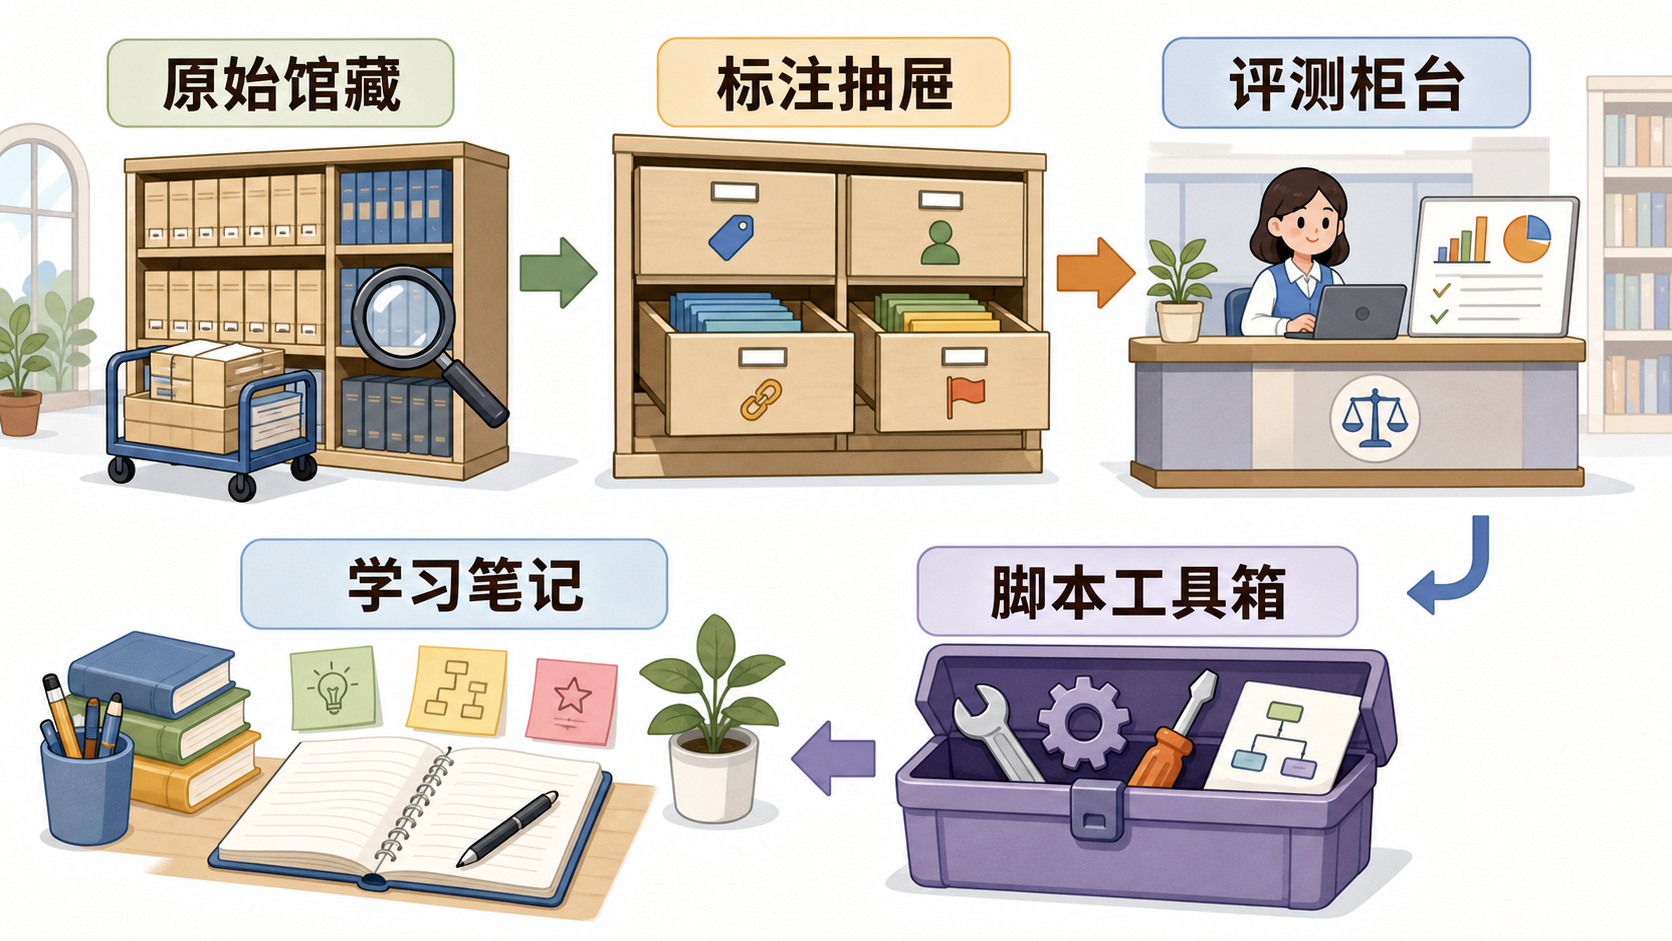
\includegraphics[width=0.96\linewidth]{assets_v2/archive_metaphor.png}
  \caption{目录不是随机堆放的：它更像一个档案馆，每个房间放一种材料。}
\end{figure}

\begin{longtable}{>{\ttfamily}p{0.28\linewidth}p{0.24\linewidth}p{0.38\linewidth}}
\toprule
\normalfont 真实目录或文件 & 费曼比喻 & 你该怎么理解 \\
\midrule
ECB+\_LREC2014/ & 原始馆藏 & 原始 ECB+ 语料，像还没加工的新闻档案。 \\
annotated\_data/ & 贴好便签的档案 & ESC 标注数据，里面标了事件和情节关系。 \\
evaluation\_format/ & 考试标准答案柜台 & 已经整理成评测脚本容易读取的格式。 \\
ecb+\_naf/ & 语言学工具卡片 & 提供 lemma、句子等信息，PPMI 基线会用。 \\
ppmi\_events\_ecb+\_test/ & 实验材料盒 & PPMI 基线相关的测试或中间材料。 \\
create\_gold\_document.py & 档案整理员 & 把原始标注整理成标准答案文件。 \\
baseline\_*.py & 答题学生 & 用规则猜事件关系，生成系统答案。 \\
eval\_script.py & 批卷老师 & 对照标准答案，计算精确率、召回率、F1。 \\
\bottomrule
\end{longtable}

\section{XML 标注到底是什么}

\begin{figure}[H]
  \centering
  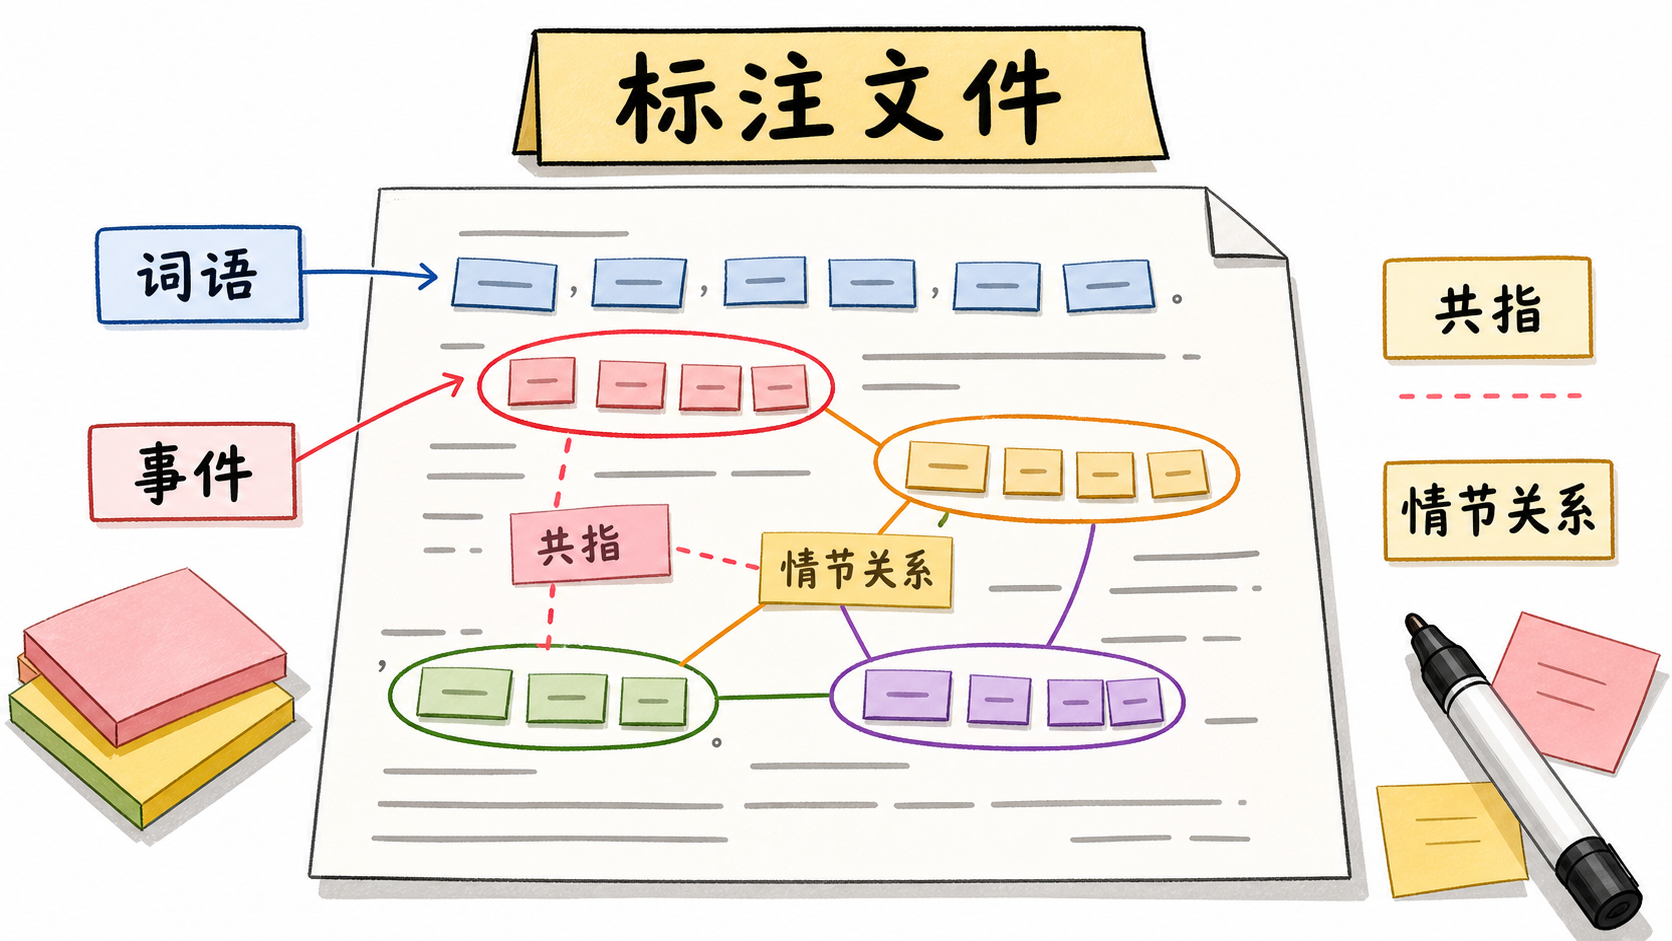
\includegraphics[width=0.96\linewidth]{assets_v2/annotation_metaphor.png}
  \caption{XML 标注可以理解成“贴满便签的新闻稿”：哪些词是事件，哪些事件互相有关，都写在便签里。}
\end{figure}

不用先害怕 XML。你可以把一个 XML 文件想成一张新闻稿，旁边贴了很多便签：

\begin{itemize}[leftmargin=2em]
  \item \textbf{token}：新闻稿里的每个词，像一个小卡片。
  \item \textbf{Markables}：哪些词被圈出来了，比如“爆炸”“逮捕”“宣布”。
  \item \textbf{Relations}：被圈出来的东西之间有什么关系。
  \item \textbf{PLOT\_LINK}：故事线关系，比如一个事件是另一个事件的前提或后续。
\end{itemize}

\begin{figure}[H]
\centering
\begin{tikzpicture}[
  font=\small,
  card/.style={draw=line, fill=paper, rounded corners=3pt, minimum width=22mm, minimum height=8mm, align=center},
  tag/.style={draw=orange!70!black, fill=softyellow, rounded corners=3pt, align=center, inner sep=5pt},
  arr/.style={-{Stealth[length=2mm]}, thick}
]
\node[card] (w1) {词1};
\node[card, right=4mm of w1] (w2) {词2};
\node[card, right=4mm of w2] (w3) {事件词};
\node[card, right=4mm of w3] (w4) {词4};
\node[tag, below=8mm of w3] (m) {Markable\\圈出事件};
\node[tag, right=18mm of m] (r) {Relation\\连接事件};
\draw[arr, blue] (m) -- (w3);
\draw[arr, orange] (m) -- (r);
\end{tikzpicture}
\caption{XML 的关键不是尖括号，而是“词、事件标注、关系标注”三层。}
\end{figure}

\section{三种数据版本像三本教材}

\begin{figure}[H]
  \centering
  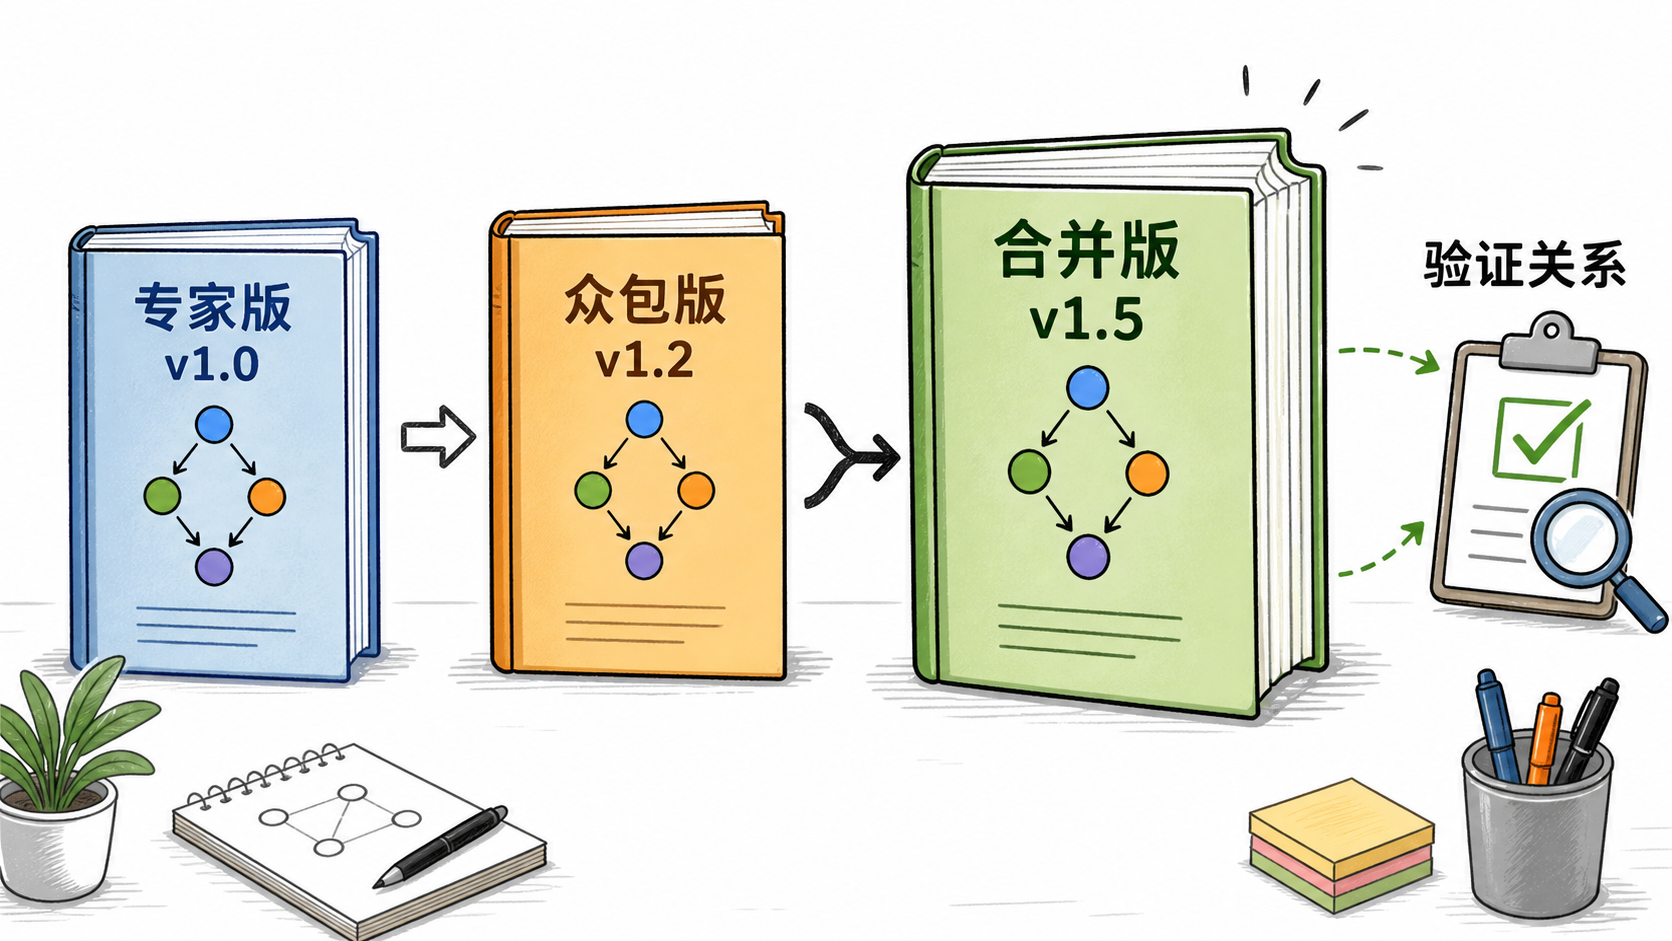
\includegraphics[width=0.96\linewidth]{assets_v2/version_metaphor.png}
  \caption{v1.0、v1.2、v1.5 可以先理解成三本不同来源的故事线教材。}
\end{figure}

\begin{itemize}[leftmargin=2em]
  \item \code{v1.0}：专家版。可以理解成老师亲自批注的版本。
  \item \code{v1.2}：众包版。可以理解成很多同学一起标注后汇总的版本。
  \item \code{v1.5}：合并版。把专家和众包信息结合起来，README 里提到还带有 \code{origin} 和 \code{validated} 这样的属性。
\end{itemize}

如果你只是学习项目结构，建议先看 \code{v1.5}，因为它更完整。

\section{标准答案是怎么做出来的}

\code{create\_gold\_document.py} 像一个档案整理员。它同时打开两类档案：

\begin{itemize}[leftmargin=2em]
  \item ECB+ 原始文件：告诉你事件 mention 和共指链。
  \item ESC 标注文件：告诉你事件之间的 \code{PLOT\_LINK}。
\end{itemize}

然后它做一件很重要的事：\textbf{把一个事件关系扩展到共指链里的更多事件提及对。}

\begin{figure}[H]
\centering
\begin{tikzpicture}[
  font=\small,
  box/.style={draw=line, fill=paper, rounded corners=3pt, minimum width=29mm, minimum height=10mm, align=center},
  data/.style={draw=blue!50, fill=softblue, rounded corners=3pt, minimum width=32mm, minimum height=10mm, align=center},
  script/.style={draw=green!60!black, fill=softgreen, rounded corners=3pt, minimum width=35mm, minimum height=10mm, align=center},
  arr/.style={-{Stealth[length=2mm]}, thick}
]
\node[data] (ecb) {ECB+\\事件和共指};
\node[data, below=8mm of ecb] (esc) {ESC\\故事线关系};
\node[script, right=18mm of $(ecb)!0.5!(esc)$] (s) {整理员脚本\\\code{create\_gold}};
\node[box, right=18mm of s] (out1) {标准答案\\事件对文件};
\node[box, below=8mm of out1] (out2) {标准答案\\共指扩展文件};
\draw[arr, blue] (ecb) -- (s);
\draw[arr, blue] (esc) -- (s);
\draw[arr, green!60!black] (s) -- (out1);
\draw[arr, green!60!black] (s) -- (out2);
\end{tikzpicture}
\caption{标准答案不是凭空来的，而是由 ECB+ 的共指信息和 ESC 的故事线标注合并出来的。}
\end{figure}

\section{基线脚本像学生做题}

基线系统不是神经网络模型。它更像学生用一套简单规则做题：

\begin{itemize}[leftmargin=2em]
  \item \code{baseline\_OP.py}：看到同一句里有多个事件，就把它们两两连起来。
  \item \code{baseline\_PPMI1.py}：看事件词的共现强度，觉得常一起出现的事件更可能有关系。
  \item \code{baseline\_PPMI\_CONTAINS.py}：在 PPMI 的基础上，又看这些事件是不是被同一个时间锚装在一起。
\end{itemize}

\begin{figure}[H]
\centering
\begin{tikzpicture}[
  font=\small,
  box/.style={draw=line, fill=paper, rounded corners=3pt, minimum width=32mm, minimum height=10mm, align=center},
  arr/.style={-{Stealth[length=2mm]}, thick}
]
\node[box, fill=softblue] (easy) {最朴素规则\\同句事件两两连};
\node[box, fill=softyellow, right=12mm of easy] (ppmi) {统计规则\\看 PPMI 共现};
\node[box, fill=softgreen, right=12mm of ppmi] (time) {加强规则\\加入时间锚};
\draw[arr, orange] (easy) -- (ppmi);
\draw[arr, orange] (ppmi) -- (time);
\end{tikzpicture}
\caption{三类基线可以按“简单规则、统计规则、时间增强规则”来理解。}
\end{figure}

\section{评测脚本像老师批卷}

\begin{figure}[H]
  \centering
  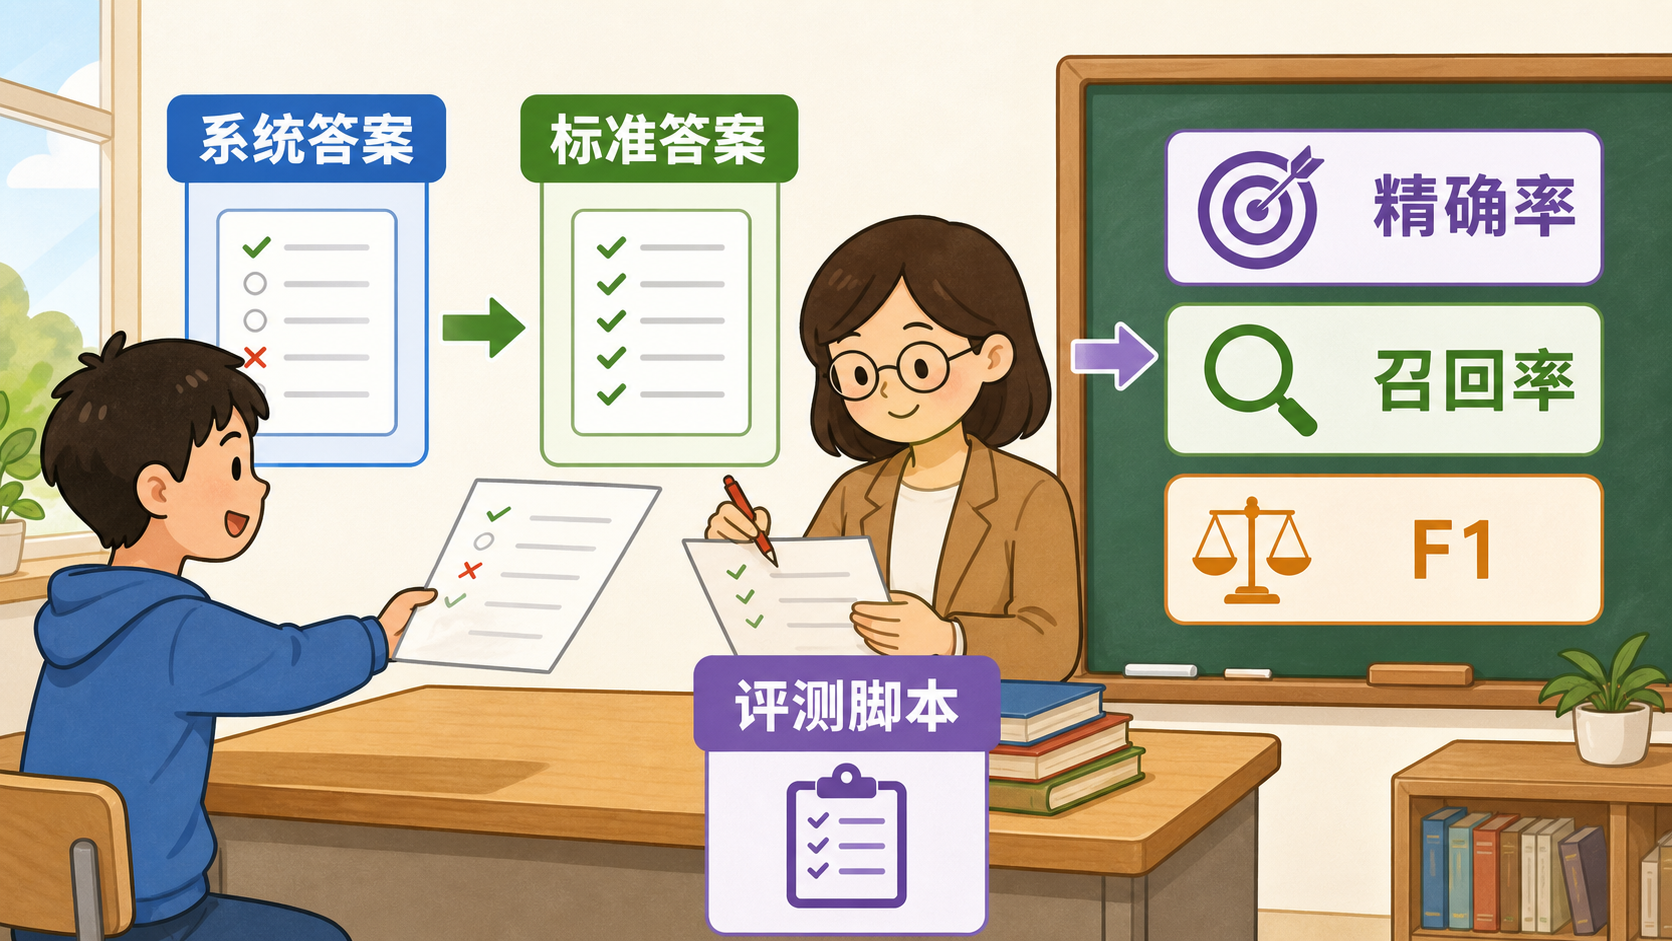
\includegraphics[width=0.96\linewidth]{assets_v2/evaluation_metaphor.png}
  \caption{系统输出像学生答案，标准答案像参考答案，评测脚本就是批卷老师。}
\end{figure}

\code{eval\_script.py} 做的事情很朴素：

\begin{enumerate}[leftmargin=2em]
  \item 读标准答案文件。
  \item 读系统输出文件。
  \item 看系统猜对了多少、猜错了多少、漏掉了多少。
  \item 算精确率、召回率、F1。
\end{enumerate}

\begin{center}
\begin{tikzpicture}[
  font=\small,
  metric/.style={draw=line, rounded corners=3pt, minimum width=35mm, minimum height=10mm, align=center},
  arr/.style={-{Stealth[length=2mm]}, thick}
]
\node[metric, fill=softblue] (p) {精确率\\猜出来的有多少是真的};
\node[metric, fill=softgreen, right=8mm of p] (r) {召回率\\真的里面找回了多少};
\node[metric, fill=softyellow, right=8mm of r] (f) {F1\\两者的折中分};
\end{tikzpicture}
\end{center}

\section{建议你按这个顺序读}

\begin{enumerate}[leftmargin=2em]
  \item \textbf{先看评测文件}：打开 \code{evaluation\_format/test\_corpus/v1.5/event\_mentions\_extended/}，感受一行三列长什么样。
  \item \textbf{再看批卷老师}：读 \code{eval\_script.py}，因为它短，而且会告诉你“系统答案应该长什么样”。
  \item \textbf{再看最简单学生}：读 \code{baseline\_OP.py}，理解同句事件配对。
  \item \textbf{再看档案整理员}：读 \code{create\_gold\_document.py}，理解标准答案怎样生成。
  \item \textbf{最后看高级学生}：读 \code{baseline\_PPMI1.py} 和 \code{baseline\_PPMI\_CONTAINS.py}。
\end{enumerate}

\section{一张总复习图}

\begin{figure}[H]
\centering
\begin{tikzpicture}[
  font=\small,
  box/.style={draw=line, fill=paper, rounded corners=4pt, minimum width=31mm, minimum height=11mm, align=center},
  arr/.style={-{Stealth[length=2mm]}, thick}
]
\node[box, fill=softblue] (raw) {原始语料\\像新闻档案};
\node[box, fill=softyellow, right=10mm of raw] (ann) {标注数据\\像便签};
\node[box, fill=softgreen, right=10mm of ann] (gold) {评测格式\\像标准答案};
\node[box, fill=softyellow, below=12mm of gold] (base) {基线脚本\\像学生作答};
\node[box, fill=softblue, left=10mm of base] (sys) {系统输出\\像学生答案};
\node[box, fill=softgreen, left=10mm of sys] (eval) {评测脚本\\像老师批卷};
\draw[arr, blue] (raw) -- (ann);
\draw[arr, blue] (ann) -- (gold);
\draw[arr, orange] (gold) -- (base);
\draw[arr, orange] (base) -- (sys);
\draw[arr, green!60!black] (sys) -- (eval);
\draw[arr, green!60!black] (gold.south west) to[out=220,in=30] (eval.north east);
\end{tikzpicture}
\caption{记住这条链：原始语料到标注，标注到标准答案，基线生成答案，评测脚本批改。}
\end{figure}

\section{打开方式}

在 VS Code 中打开整个项目：

\begin{lstlisting}[language=bash]
code /Users/luyifeng/Documents/GitHub/EventStoryLine
\end{lstlisting}

这份费曼版文档在：

\begin{lstlisting}
yifeng_study/feynman_project_guide.tex
yifeng_study/assets_v2/
\end{lstlisting}

中文 LaTeX 建议用 XeLaTeX 编译：

\begin{lstlisting}[language=bash]
cd /Users/luyifeng/Documents/GitHub/EventStoryLine/yifeng_study
xelatex feynman_project_guide.tex
\end{lstlisting}

\end{document}
